\begin{document}

\begin{frame}{Current Progress}
    \begin{itemize}
        \item Cleaned up assets in CloudCompare
        \item Worked on pre-aligned Tikal tunnel point clouds in RealityCapture
        \item Subsampled the point cloud and generated meshes through PoissonRecon
        \item Exportable as .fbx, .obj etc.
    \end{itemize}    
\end{frame}

\begin{frame}{Renders}
    \begin{columns}
        \begin{column}{0.33\textwidth}
            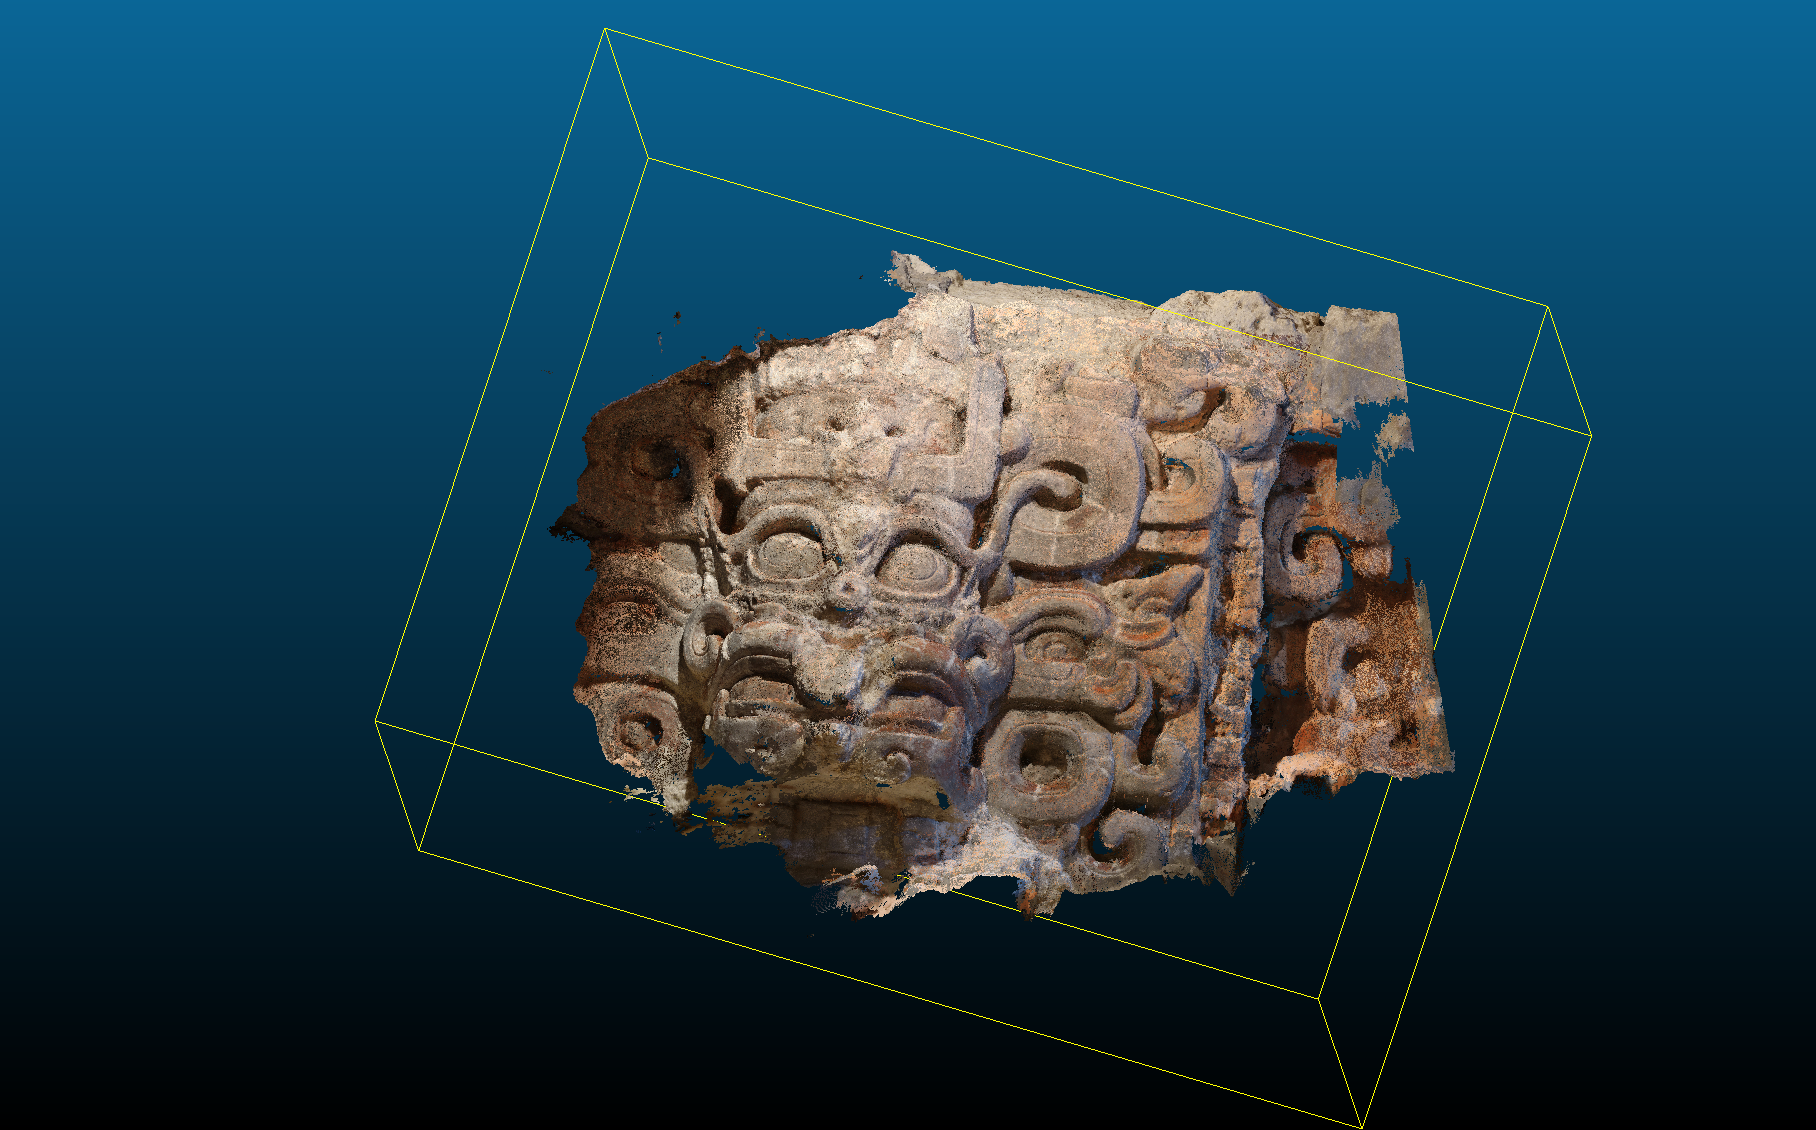
\includegraphics[height=0.7\textheight, keepaspectratio]{images/maya/capture.png}
        \end{column}
        \begin{column}{0.33\textwidth}
            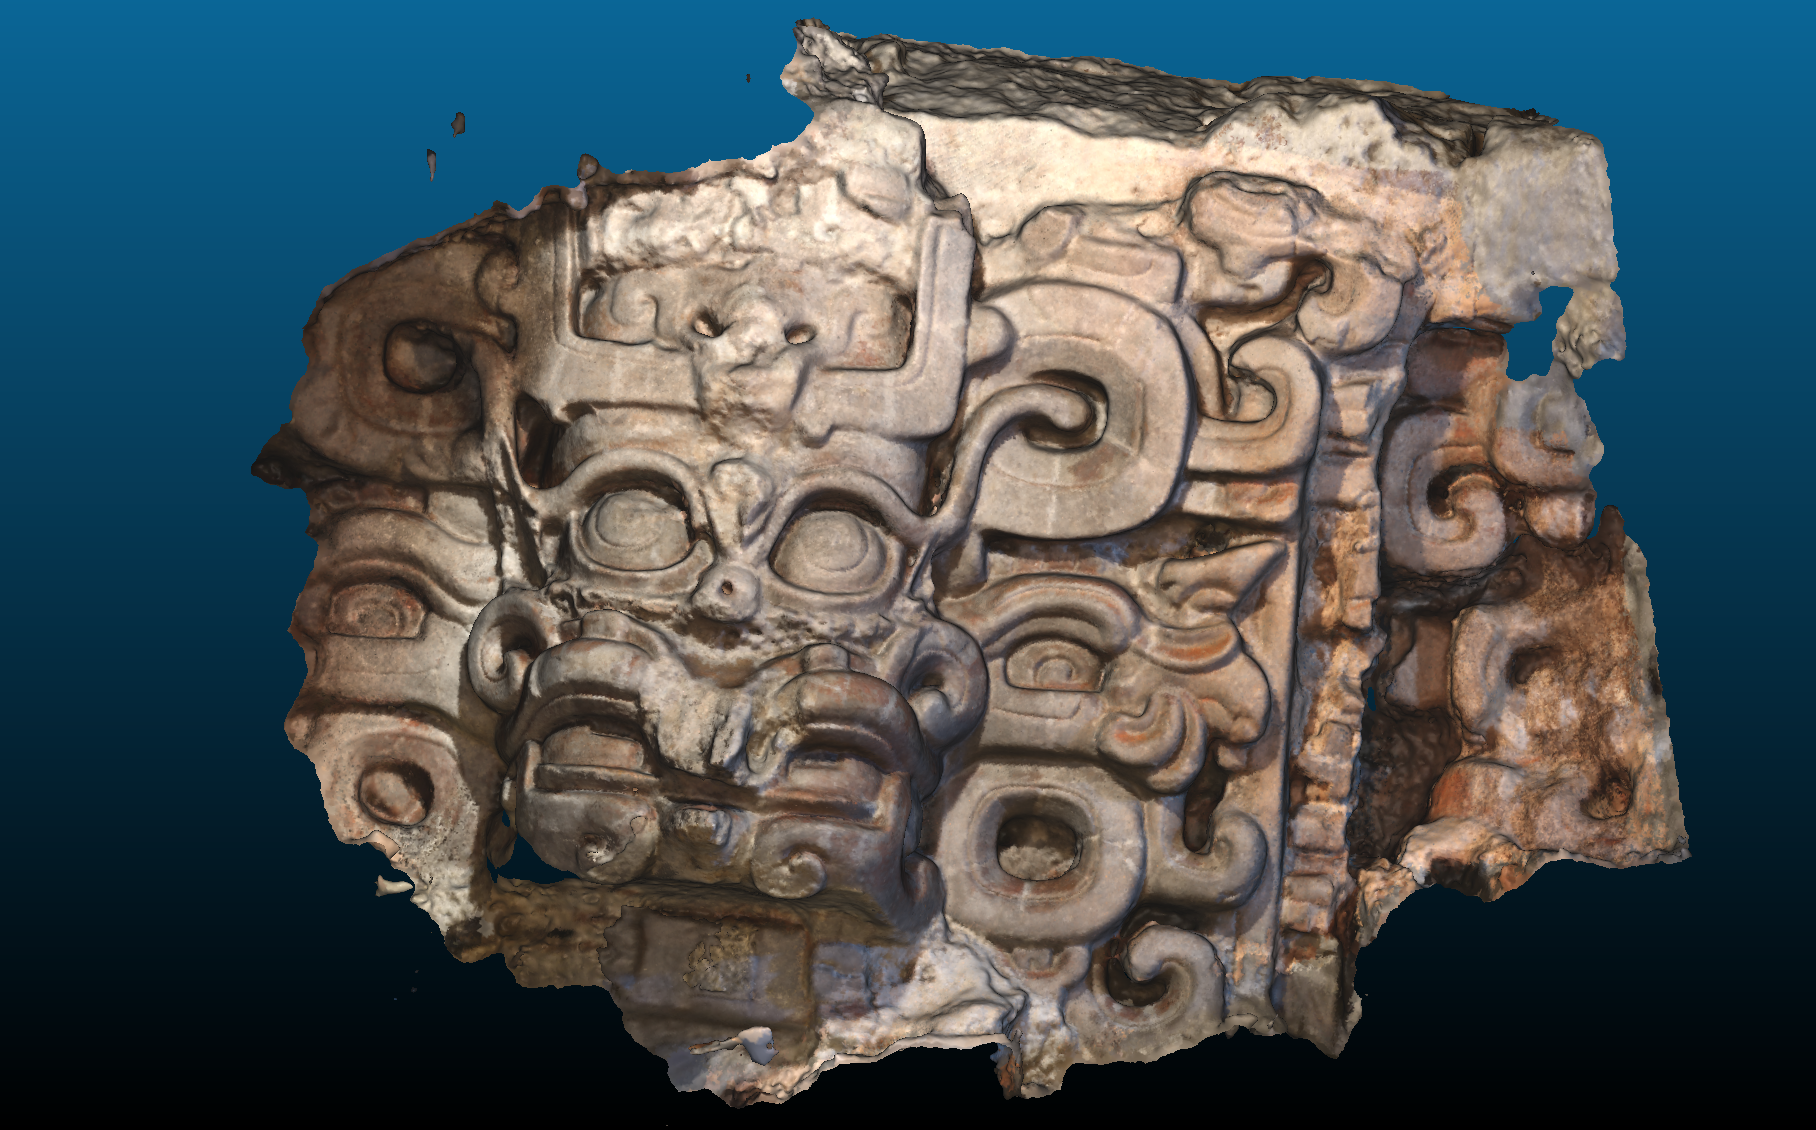
\includegraphics[height=0.7\textheight, keepaspectratio]{images/maya/capture2.png}
        \end{column}
        \begin{column}{0.33\textwidth}
            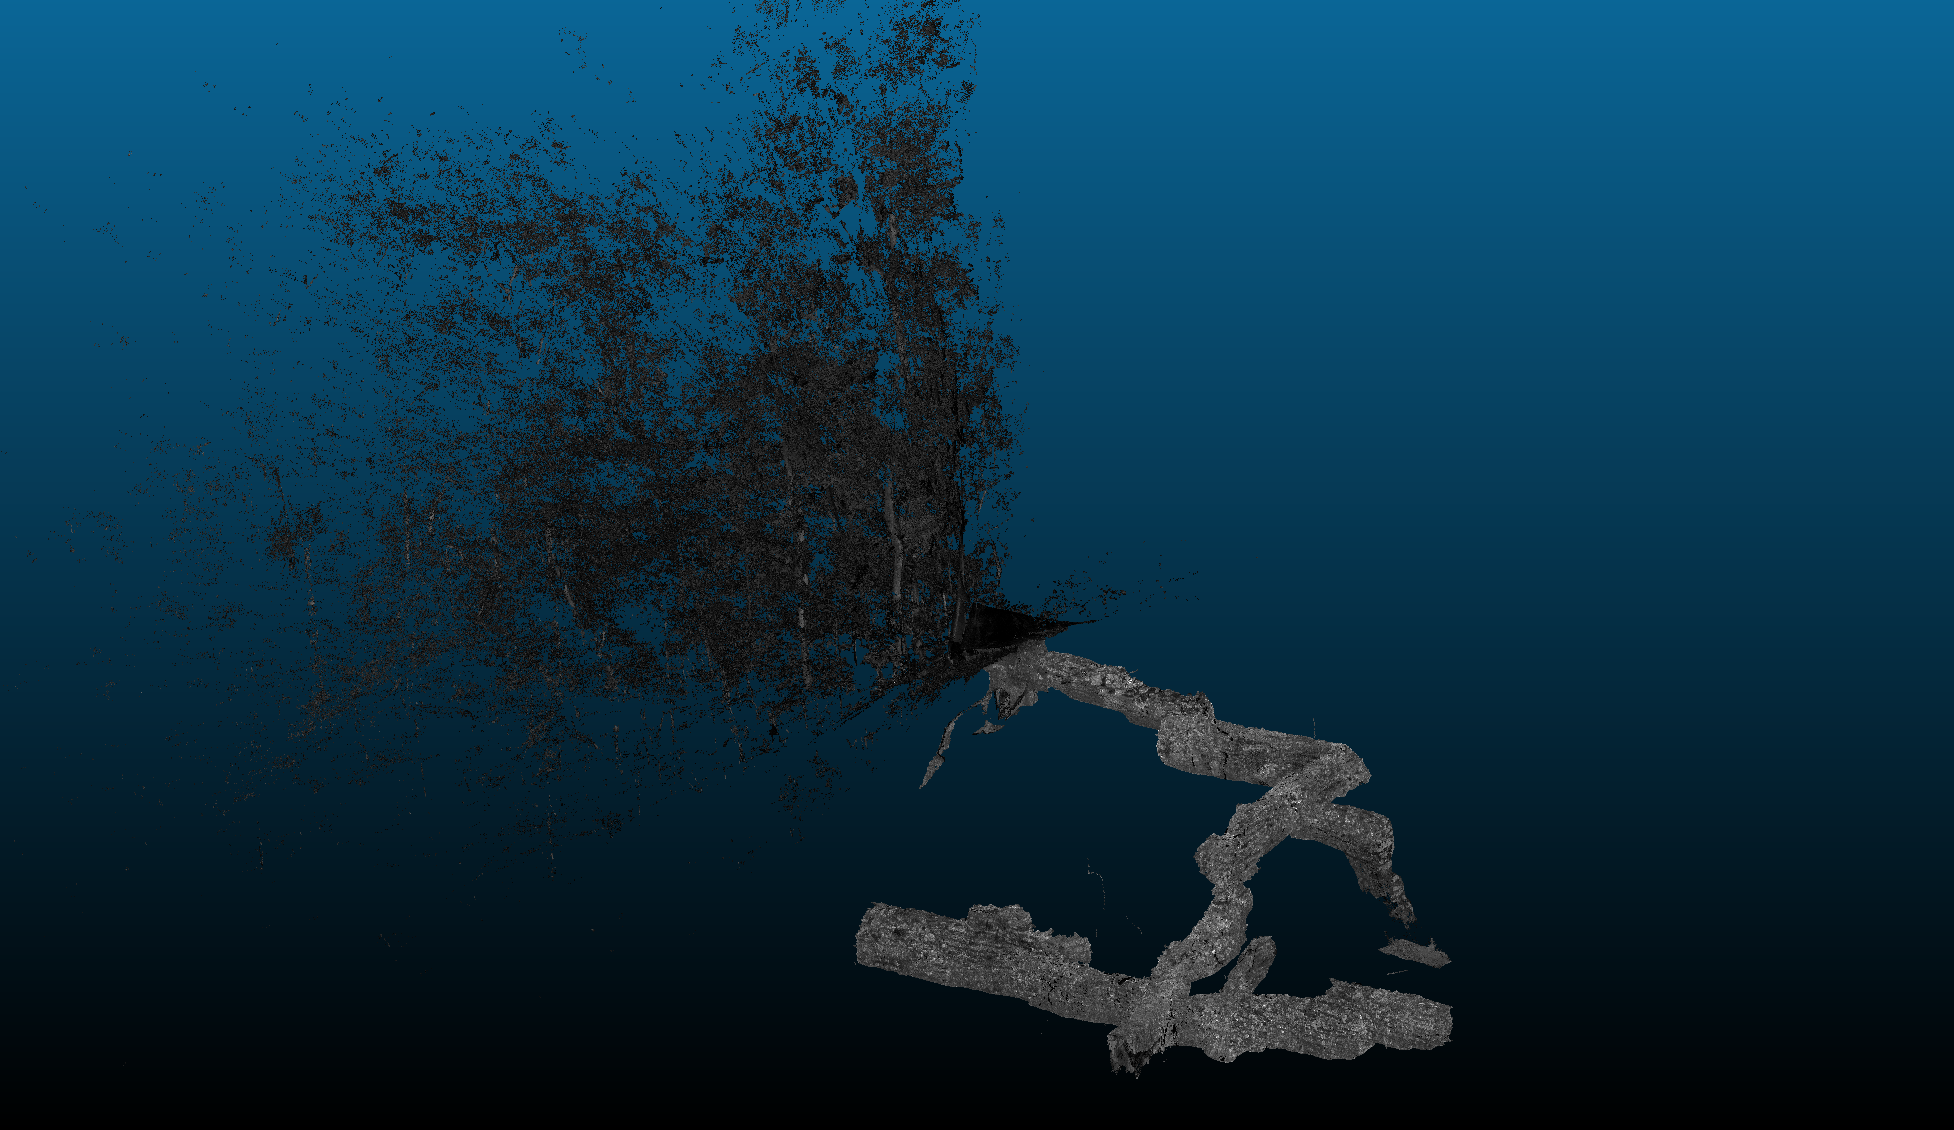
\includegraphics[height=0.7\textheight, keepaspectratio]{images/maya/capture5.png}
        \end{column}
    \end{columns}
\end{frame}

\begin{frame}{Renders}
    \begin{columns}
        \begin{column}{0.5\textwidth}
            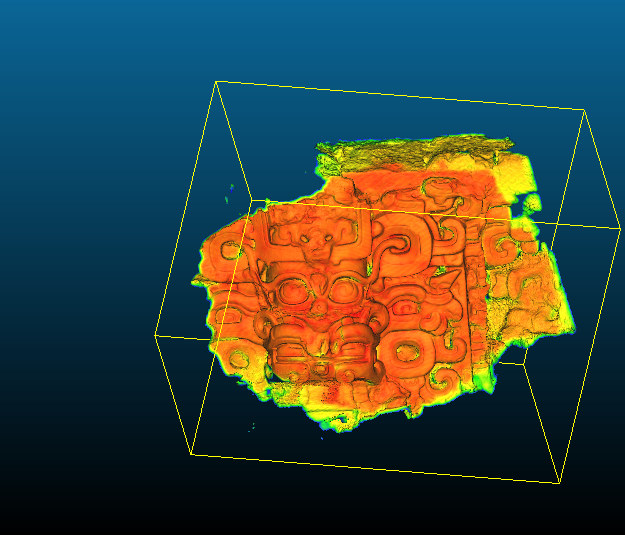
\includegraphics[height=0.7\textheight, keepaspectratio]{images/maya/capture4.png}
        \end{column}
        \begin{column}{0.5\textwidth}
            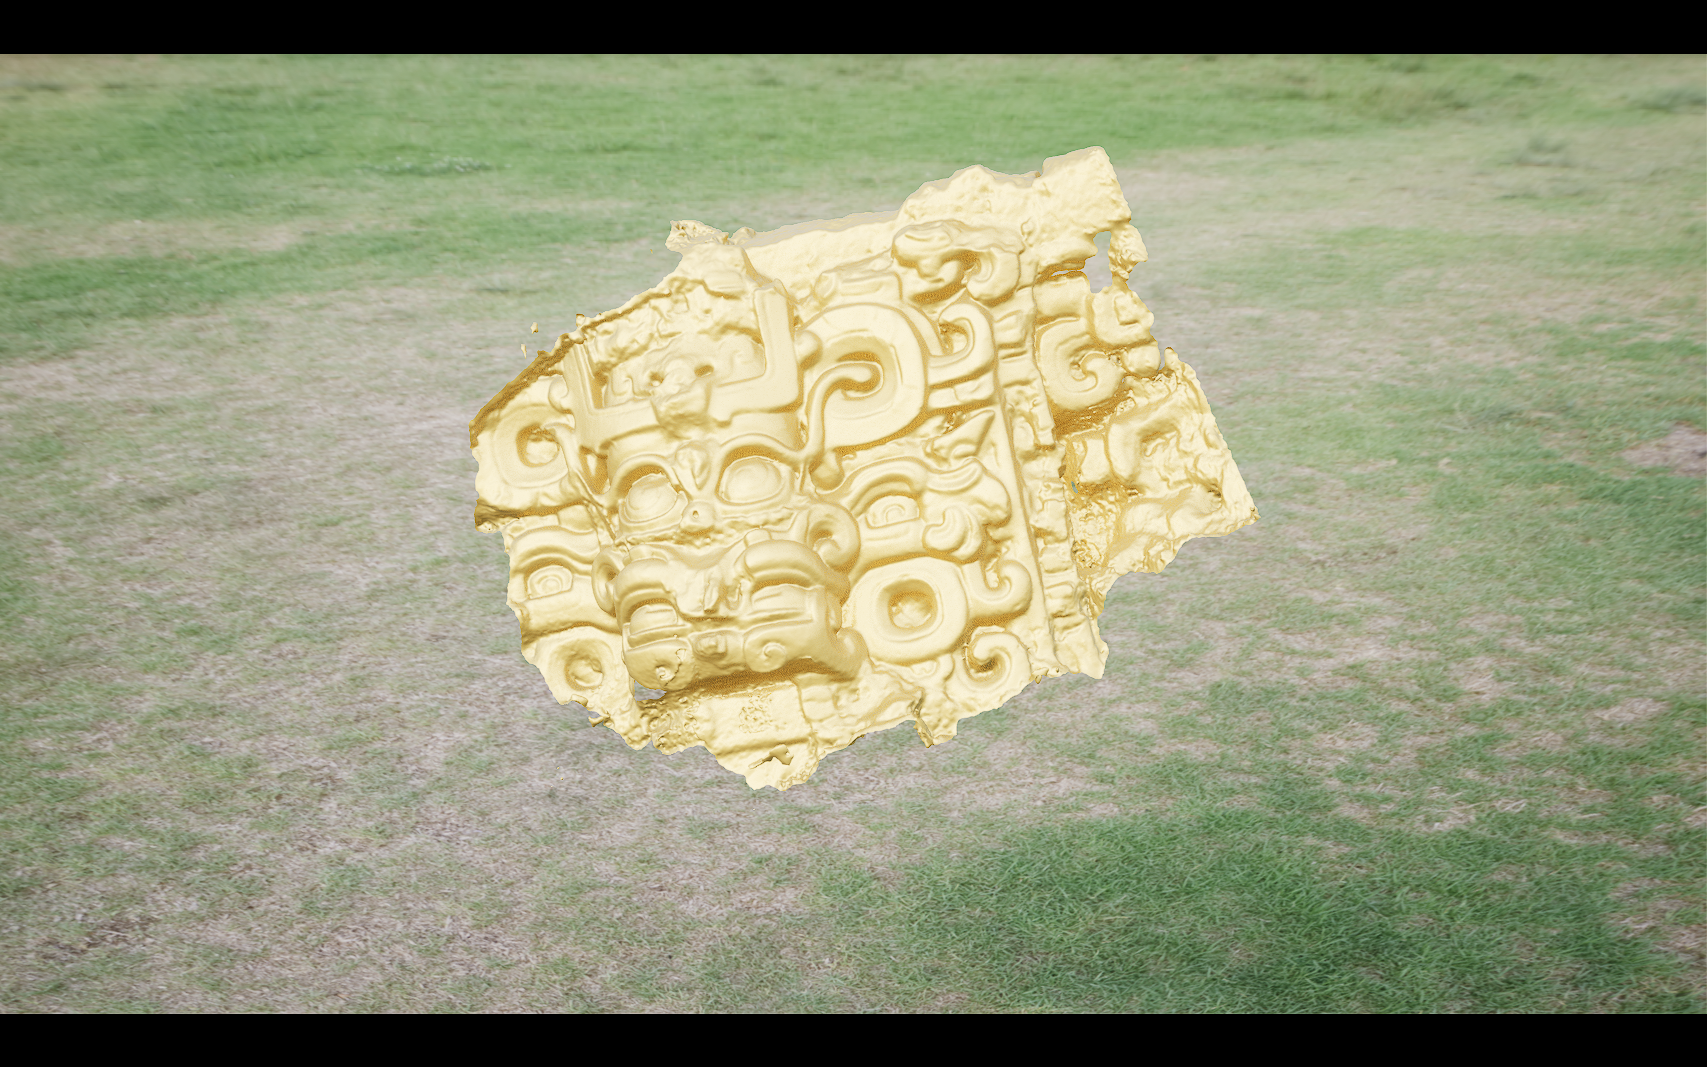
\includegraphics[height=0.7\textheight, keepaspectratio]{images/maya/render.png}
        \end{column}
    \end{columns}
\end{frame}

\begin{frame}{Next}
    \begin{itemize}
        \item Further refine and complete the asset in ZBrush.
        \item Sort the completely unsorted point clouds and align them in RealityCapture
    \end{itemize}    
\end{frame}

\end{document}
